\documentclass[12pt, letterpaper]{article}
\usepackage[utf8]{inputenc}
\usepackage[margin=1in]{geometry}
\usepackage[super]{nth}
\usepackage{hyperref}
\usepackage{lineno}
\usepackage[
singlelinecheck=false
]{caption}
\usepackage{amsmath}
\usepackage{amsfonts}
\usepackage{bm}
\usepackage{bbm}
\usepackage{graphicx}
\usepackage{csvsimple}
\usepackage[section]{placeins}
\usepackage{lineno}
\usepackage{natbib}

\title{KIN: A method to infer relatedness from low-coverage ancient DNA}
\author{Divya Ratan Popli, Stéphane Peyrégne, Benjamin M. Peter}
%\date{5 August 2021}
\linenumbers

\setlength{\parskip}{1em}
\setlength{\parindent}{0em}

\newcommand{\BZ}{\mathbf{Z}}
\newcommand{\BD}{\mathbf{D}}
\newcommand{\BN}{\mathbf{N}}
\newcommand{\BH}{\mathbf{H}}
\newcommand{\Btheta}{\pmb{\theta}}


\begin{document}

\maketitle

\begin{abstract}

\noindent Inferring familial relationships is an important question in population genetics. Knowing genetic kinship of ancient individuals leads to insights into the culture and social hierarchy of ancient populations, and is  relevant for downstream genetic analyses. However, estimating relatedness from ancient DNA is difficult since DNA sequences extracted from ancient remains may have low coverage, ascertainment bias, or contamination from various sources. 

Here, we present KIN, a Hidden-Markov-Model-based approach to identify identity-by-descent fragments and to estimate degree of relatedness. KIN can accurately determine up to 3rd-degree relatives and differentiate between sibling and parent-child relationships using ancient DNA sequence data with as little as 0.05x coverage. KIN also incorporates an adjustment for contamination, and an additional model to estimate the location of long runs of homozygosity, and uses it to improve classification accuracy.

We show in simulations that KIN performs at near perfect classification accuracy at inferring first-degree relationships, and at 90\% accuracy for second degree even at 0.05x coverage.

We illustrate the utility of KIN on two applications, one on a Neandertal group from Siberia, Russia, and one in a Bronze-Age modern human population from the Lech Valley, Germany. 
We find that in both cases, KIN matches the findings of existing approaches and provides new insights. 

Thus, KIN is a useful tool for analyzing relatedness for large ancient-DNA datasets with low-coverage sequencing data that is applicable to any diploid species, without the requirement for a reference panel.
\end{abstract}

\section{Introduction}

\subsection{Why study relatedness?}

Identifying related individuals is a common task in genetic studies. Relatedness is of direct interest in e.g. DNA forensics, where familial search can aid in solving criminal cases, and to identify unknown deceased persons \cite{murphy_law_2018,ram_genealogy_2018}. Genetic paternity tests have an important application in resolving family relation, e.g. in establishing relationship between a person applying for immigration and the claimed relatives \cite{egeland_beyond_2000}. It is also an essential step in population genetics and association studies, where samples are typically assumed to be independent random draws from the population. For animal and plant breeders and conservation biologists, reconstructing pedigrees and finding related individuals is important to avoid inbreeding and ensure diversity \cite{habier_impact_2007,oliehoek_estimating_2006,kardos_measuring_2015}.

In ancient DNA studies, relatedness can be used to identify bones and teeth belonging to the same individual, and can provide an understanding of an ancient society's organization and hierarchy, social structures, and cultural aspects ~\cite{baca_ancient_2012,mittnik_kinship-based_2019,sikora_ancient_2017}.


\subsection{Approaches to estimate relatedness from high-coverage data}

Commonly, pairs of related individuals are identified by looking for parts of the genome that are identical by descent (IBD), i.e. inherited from a recent common ancestor. Due to the laws of Mendelian segregation, each parent will share exactly one set of chromosomes IBD with their offspring, while subsequent recombination means that a grandparent will, on average share a quarter of their genome with a grand-child. Along the genomes of a pair of diploid individuals, there are three IBD states possible at any given position: either no chromosomes are IBD, only one chromosome is IBD, or both chromosomes are IBD. The genome-wide proportions of these states (usually referred to as $k_0$, $k_1$, $k_2$, so that $k_0+k_1+k_2=1$) can be used to infer the degree and nature of relatedness for a pair of individuals. For example, a pair of siblings are expected to have all three possible IBD states with proportions of 0.25,0.5,0.25, respectively (Fig \ref{fig0:schematic}). These IBD probabilities can directly be used to categorize their relatedness as shown in table \ref{tab:Table 1}. One can also use these probabilities to estimate the coefficient of relatedness $r$, which is defined as the proportion of the genome that is IBD. In the absence of inbreeding, this would be calculated as $r= k_1/2 + k_2$.

However, since it is not possible to directly observe IBD segments, a common approach is to first identify segments of the genome that are Identical by State (IBS) and to use population allele frequencies obtained from a reference panel to calculate the probability of IBD given IBS. There are several methods that utilize population allele frequencies, phase information, recombination maps, or genotype calls to co-estimate IBD and the relatedness coefficient \cite{huff_maximum-likelihood_2011,li_relationship_2014,li_accurate_2014,thornton_estimating_2012, boehnke_accurate_1997,lynch_estimation_1999, albrechtsen_natural_2010, purcell_plink_2007,manichaikul_robust_2010}.

\begin{figure}[h!]
    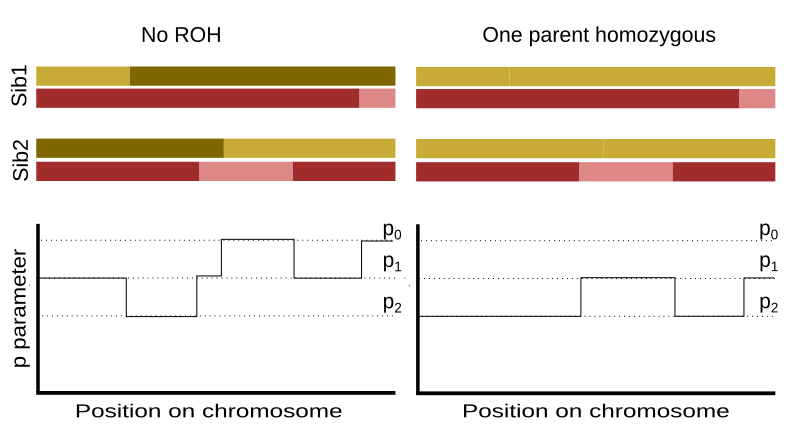
\includegraphics[width=18cm]{plots/inkscape_finalImg/schematic_sib.png}
    \centering
    \caption{IBD sharing between siblings without and with ROH. In top row, recombined chromosomes inherited from parents by a pair of siblings are shown. On the left, the parents have unrelated chromosomes, and on the right one parent has a homozygous pair of chromosomes. The bottom row shows the expected proportion of differences (p) along the chromosome in both the cases p can take values of $p_0$, $p_1$ or $p_2$ which are the expected proportion of differences in IBD states 0,1 and 2 respectively.  }
    \label{fig0:schematic}
\end{figure}


\begin{table}[h!]
\caption{\label{tab:Table 1}IBD sharing probabilities for different relations in absence of inbreeding}
\begin{tabular}{|c|c|c|c|}
    \hline
    Relatedness & $k_0$ & $k_1$ & $k_2$\\
    \hline
    Unrelated & 1 & 0 & 0\\
    \hline
    3rd Degree & 0.75 & 0.25 & 0\\
    \hline
    2nd Degree & 0.5 & 0.5 & 0\\
    \hline
    Siblings & 0.25 & 0.5 & 0.25\\
    \hline
    Parent-Child & 0 & 1 & 0\\
    \hline
    Identical/twins & 0 & 0 & 1\\
    \hline
\end{tabular}
\label{table1}
\end{table}

\subsection{Approaches that address problems with ancient DNA data}
One major issue with applying the above-mentioned methods to ancient DNA data is that the sequence coverage is typically low, making it difficult to generate accurate genotype calls.
Several methods surmount this problem by using genotype likelihoods \cite{lipatov_maximum_2015,korneliussen_ngsrelate_2015}. In this way, it is possible to account for the uncertainty in genotype calls by summing over all possible genotypes weighted by their genotype likelihoods. However, these approaches typically still require at least 2x coverage, since genotype likelihoods may be imprecise at lower coverages \cite{korneliussen_angsd_2014} . Ancient DNA analyses often face additional challenges such as contamination with present-day DNA \cite{peyregne_present-day_2020-1}, absence of suitable reference panels, and ascertainment bias in the case of data generated from DNA capture \cite{prufer_computational_2010, vai_kinship_2020}.

Several methods have been proposed to estimate relatedness without a reference panel, but many of these require either $>4$x coverage \cite{waples_allele_2019}, or a large sample size to get an estimate of allele frequencies in the population from which the sampled individuals originate \cite{theunert_joint_2017}. A second issue is contamination. If the contamination stems from another population, contaminated data will look more dissimilar to other individuals from the analyzed population, and hence relatedness inference will be biased towards  less relatedness.  In addition, some analyzed  genomes  may have long runs of homozygosity (ROH), for example due to a small population size, or recent inbreeding. Long ROH cause related individuals to seem genetically more similar to each other, but do not affect the genetic distance between unrelated individuals.

Moreover, ancient DNA is commonly captured with a SNP array that enrich for informative variants. Particularly methods based on the fraction of sites in different IBS states are sensitive to the ascertainment bias caused by this non-random selection of targetted sites \cite{waples_allele_2019}. 

READ \cite{kuhn_estimating_2018} addresses several of the issues encountered in the analysis of ancient DNA. In particular, the lack of  genotype calls is dealt with by randomly sampling alleles from each individual. A string of these alleles at each position (called pseudo-haploids) are then compared to other individuals to calculate average pairwise genetic distances, which in turn are used to infer relatedness. However, READ only infers the degree of relatedness, and only up to second degree.

\subsection{How our method works}
Here, we present KIN (Kinship INference), a Hidden Markov Model (HMM)-based approach to estimate relatedness and IBD from low-coverage ancient DNA data. KIN can detect up to \nth{3}-degree relatives, and differentiates between siblings and parent-child relationships. KIN is also able to take into account ROH, contamination and ascertainment. We validate the performance of KIN using simulations and show that we are able to infer relatedness in real data from two datasets: a group of Neandertals and a group of Bronze age individuals.


\section{New Approaches}\label{new_approaches}

To infer the case of relatedness, KIN fits one HMM for each pair of individuals and for each possible relatedness case. The KIN-HMM infers IBD sharing between a pair of low-coverage individuals, optionally taking ROH tracts and contamination estimates in each individual into account. The best-fit model is then assigned as the inferred relatedness. If the locations of ROH tracts are unknown, we provide another HMM (ROH-HMM) to coarsely estimate the location of ROH for samples with sufficient coverage ($\geq 0.1x$). Our method is available on \url{https://github.com/DivyaratanPopli/KIN_snakemake} along with a \texttt{snakemake} \cite{koster_snakemakescalable_2012} pipeline to generate the input files for the models directly from bam files. 


\subsection{Model description}\label{method_overview} 

The goal of KIN-HMM is to infer how two individuals are related via the patterns of shared IBD-states along a pair of genomes. For this purpose,  we subdivide the genomes of a pair of individuals into $L$ large genomic windows (typically of size 10Mb), and infer the pattern of IBD-sharing for each relatedness case we consider (Unrelated, $5^{th}$ Degree, $4^{th}$ Degree, $3^{th}$ Degree, Grandparent-Grandchild, Avuncular, Half-siblings, Parent-Child, Siblings, and Identical). We then compare the likelihood between all models, and classify each pair to the model with the highest likelihood. We also return the most likely locations of IBD tracts (using standard Viterbi algorithm), and the state posterior probabilities $\BZ$. 

The details of the likelihood computation are given in section \ref{ll}. As is the case for any HMM, KIN-HMM requires a set of emission (section \ref{B}) and transition probability matrices. We assume the transition matrix for each relatedness case is fixed. Our emissions include a vector of parameters ($\delta$) that describe the variance in the data for each IBD state that we infer from the data (section \ref{B}).



\subsection{Input of KIN-HMM}\label{hmm_input}
The inputs of our algorithm are i) the number of overlapping sites for the $w$-th window $N_w$ for which both samples have at least one read available, ii) the expected number of pairwise differences $D_w$ at these sites, and iii) the probability of ROH in windows, by default obtained from ROH-HMM described in section \ref{roh}.

$D_w$ is the number of sites that are different between a pair of individuals. For high-coverage data, this can be estimated accurately by comparing genotypes, but for low-coverage samples, $D_w$ needs to be estimated. The simplest approach is to  randomly-sample a read from each position to make "pseudo-haploid" sequences \cite{haak_massive_2015}. However, such an approach may result in loss of data, and hence we calculate $D_w$ by implicitly summing over all possible samplings:
\begin{align}\label{eq:x}
D_w &= \sum_{s=1}^{N_w} \nu_i(s) (1-\nu_j(s)) + (1-\nu_i(s)) \nu_j(s)
\end{align}
Here, $\nu_i(s)$ and $\nu_j(s)$ are the proportions of reads carrying the derived allele at SNP index $s$ for individuals i and j respectively.
Throughout, we will use bold-face notation to refer to the vector (or matrix) collecting  all the terms, e.g. $\BD = (D_1, D_2, \dots D_L)$. 


\subsection{Log likelihood of the KIN-HMM}\label{ll}
The KIN-HMM uses $\BD$ and $\BN$ to classify each window into three hidden states $Z_w \in$ ($0$, $1$, $2$), reflecting zero, one or two shared chromosomes IBD, respectively. To take ROH into account, we define the variable $H_w \in$ ($0$, $1$, $2$) that designates that zero, one or both individuals are homozygous in window $w$. Since $H_w$ is unobserved, in practice we use the estimates from ROH-HMM: $h_{wj} = P(H_w = j)$. 

There are three additional model parameters, $\pi, \mathbf{A}$ and $\delta$. The initial probabilities $\pi$ give the probabilities of being in each state $Z_0$ (at the beginning of each chromosome), which we set to uniform for simplicity. The transition matrix $\mathbf{A}$ gives the probability of moving from state $i$ to state $j$, given by $a_{ij}$, and is fixed and estimated from simulations for each relatedness case. The overdispersion-parameter $\delta$ takes into account that SNPs in each window vary in their allele frequency (see next setion).  For compactness of notation, we group the fixed parameters: $\theta = (\BN, \mathbf{A}, \pi)$. 

Thus, the complete data likelihood for the HMM is

\begin{align}\label{eq:1}
\log P(\BD,\BZ|\BH, \theta, \delta) &= \log P(\BD|\BZ,\BH, \theta, \delta) + \log P(\BZ |\theta) \nonumber\\
&= \sum_w \log P(D_w|Z_w,H_w, N_w, \delta) + \sum_w \log P(Z_w |Z_{w-1},A) + \log P(Z_0|\pi)\text{.}
\end{align}

Here, $\BZ$ is not dependent on $\BH$, $\theta$ and $\delta$.

\subsection{Emission probability}\label{B}

Using this setup, we can isolate the emissions $P(D_w | Z_w, H_w ,\theta, \delta)$ from equation \ref{eq:1} and optimize them for $\delta$. The simplest model is to assume that sites in each window are equally distributed and independent, in this case we could use the  binomial likelihood:
$$P(D_w|Z_w, H_w, N_w) \sim \text{Binom}[D_w ; p(Z_w, H_w), N_w] \text{,}$$

where, $p$ is the proportion of differences expected for a particular IBD and ROH state. If the two individuals are unrelated in a particular window (i.e. $Z_w = 0$), then the expected proportion of pairwise differences depends solely on the population history, and we denote this proportion with $p_0$. If the two individuals share one or even both copies of the genome IBD, we would expect the proportion of differences to be reduced to $p_1 = \frac{3}{4} p_0$, and $p_2 = \frac{1}2 p_0$, respectively, since either one or two of the four possible comparisons will be between identical chromosomes \cite{kuhn_estimating_2018}. Thus, $p(Z_w=i, H_w=0) = p_i$.

The proportion of differences between unrelated individuals $p_0$ is an important parameter. We follow READ \cite{kuhn_estimating_2018} and estimate $p_0$ as the median of differences for all possible pairs of individuals, which should work well if the majority of individuals in the samples are unrelated.

The presence of inbreeding adds an additional complication, as the number of shared chromosome may change. For example, when considering two bones from the same individual, we would expect the entire genome to have a pairwise difference of $p_2$, because two out of the four compared chromosomes are between identical copies. However, in inbred regions all four chromosomes will be identical, and so the expected pairwise differences are zero ($p_3$ in equation \ref{eq:2}). Note however, that $p_0$ does not depend on the presence of ROH, since all comparisons are between unrelated chromosomes even if both individuals are homozygous at a particular locus. 

Taken together, we can summarize $p$ in the following matrix, where rows give the state of $Z_w$, and columns of $H_w$:
\begin{equation}\label{eq:2}
    p(Z_w, H_w) = \left[\begin{array}
{rrr}
p_0 & p_0 & p_0 \\
p_1 & p_2 & p_3 \\
p_2 & p_3 & p_3
\end{array}\right]
\end{equation}

As explained above, $p_3 = 0$. However, as we do all our calculations in large windows, the start/end positions of windows may not coincide with that of ROH tracts, and we found that we obtain better results by setting $p_3 = \frac{p_2}{2}$.

The effect of these considerations is that even though we have nine possible combinations of $Z_w$ and $H_w$ for each window, there are actually only four unique $p$-parameters $p_i$ with $i$ $\in$ (0,1,2,3). 

\paragraph{Beta Binomial Model}
The Binomial Model laid out above assumes that sites are independent. However, due to genetic linkage, nearby sites will be correlated. As a result, we empirically find that the data often has considerably higher variance than would be expected from a binomial model (fig. S\ref{figS1:binom}). We take this into account by adding an overdispersion parameter $\delta$. Just like $p(Z_w,H_w)$, $\delta(Z_w,H_w)$ depends on the number of chromosomes compared, and so each of the  four $p_i$ has a corresponding $\delta_i$ parameter. 

Taken together, our emission probabilities are 
\begin{align}\label{eq:3}
P(D_{w}|Z_w,H_w,N_w, \delta) &\sim BB[D_w; p_i, \delta_i, N_w] \nonumber\\
&= \binom{N_w}{D_w}\frac{B(D_w+p_i \delta_{i}, N_w-D_w+ \delta_{i}(1-p_{i}))}{ B(p_{i}\delta_{i}, (1-p_{i})\delta_{i})},
\end{align}
where $i$ is fully determined by the combination of $Z_w$ and $H_w$ (see equation \ref{eq:2}).

This parameterization of the beta distribution in terms of expected value $p$ and overdispersion $\delta$ is also called the Balding-Nichols-model \cite{balding_method_nodate}, and is distinct from the more common parametrization in terms of $\alpha$ and $\beta$. We use this equation even if preprocessing steps result in non-integer $D_w$ and $N_w$, in which case we approximate the binomial coefficient using Gamma functions.   

\subsection{Estimation of $\delta$}\label{delta}
We estimate the $\delta$-parameters using an Expectation-Maximization (EM) algorithm (REF). In an EM-algorithm, we iterate the Expectation and Maximization steps until the algorithm converges.

\paragraph{Initialization}
The value of $\delta_i$ is unknown to start with, and we set it to a random value between 0 and 1000.

\paragraph{Expectation step}
In the $t$-th iteration, we calculate the posterior probability of each IBD state in each window $\gamma^{(t)}_{wi} = P(Z_w=i | D_w, H_w, \theta_i, \delta_i^{(t)})$ using the forward-backward algorithm, where $\delta_i^{(t)}$ is the current guess for $\delta$ for a given IBD state.

\paragraph{Maximization step}
The only free parameters we estimate in the M-step are the overdispersion parameters $\delta_i$. We do this optimization using a cost function, which is the log-emission probability weighted by the posterior probabilities of the hidden states $\gamma_{wj}$ and optionally the ROH state-probabilities $h_{w\omega}$ obtained from the ROH-HMM.


\begin{align}\label{eq:4}
\mathcal{C} &= \mathbb{E}[\log P(D_w|Z_w, H_w, \theta, \delta^{(t-1)}]\nonumber\\
&= \sum_{w=1}^L \sum_{j=0}^2\sum^2_{\omega=0} \log P(D_{w}|N_w, \delta_{j \omega}^{(t-1)}, p_{j \omega})h_{w\omega}\gamma_{wj}
\end{align}


Using equation \ref{eq:2}, we simplify this by grouping all the terms that would result in the same $p_i$ and $\delta_i$, i.e.

\begin{align*}\label{eq:5}
g_{w0} &= \gamma_{w0}\\
g_{w1} &= \gamma_{w1} h_{w0}\\
g_{w2} &= \gamma_{w2} h_{w0} + \gamma_{w1} h_{w1}\\
g_{w3} &= \gamma_{w2} h_{w1} + \gamma_{w2} h_{w2} + \gamma_{w1} h_{w2}
\end{align*}

So we can rewrite equation \ref{eq:4} as:
\begin{align}\label{eq:6}
\mathcal{C} &= \sum_{i=0}^3 \sum_{w=1}^L \log P(D_{w}|N_w, \delta_i, p_i)g_{wi}
\end{align}

The cost function \ref{eq:6} has one independent term for each $i$ and so we can separate them and estimate each $\delta_i$ independently using the minimize\_scalar algorithm implemented in \texttt{scipy.optimize} \cite{virtanen_scipy_2020}. 

%\paragraph{Constraints on $\delta$ optimization}\label{delta_constraint}

Unconstrained optimization of the $\delta_i$ could result in some confounding of cases, We realized that different cases of relatedness have different number of IBD states possible. For example, siblings may have all three IBD states present while a Parent-Child has only $Z_w=1$. However, the parent-child model could fit data generated under the sibling model by assigning it a very high $\delta_1$, which would reduce performance  (for example, see fig. S \ref{figS4:bndsbeta}). We avoid this problem by constraining the $\delta$ such that the beta distributions for the different cases overlap by at most one standard deviation.

\subsection{Model comparison}\label{model_comp}
To infer the most probable relatedness case, we run our model on all relatedness cases (section \ref{method_overview}) and compare the resulting likelihoods. We output the relatedness corresponding to the maximum likelihood model, and the confidence as given by the log likelihood ratio between the two highest likelihood models. The log likelihood-ratio is commonly used in likelihood-ratio tests to compare nested models. However, in our case, models are not nested, and so standard likelihood-ratio theory does not apply. For this reason, we use the log likelihood ratio between the two best models as a statistic to assess the confidence in our classifications, and use simulations to obtain critical values (Fig S \ref{figS10:cutoff}). 

\paragraph{Grouping of cases}
Particularly for low-quality data, we may not be able to distinguish all cases. Thus, we group $4^{th}$ and $5^{th}$ degree relatives together with unrelated.  Similarly, we group  half-siblings, avuncular and grandparent-grandchild to  $2^{nd}$-degree relatives in the final results. We report the final pairwise classification in the following categories: Unrelated, Third Degree, Second Degree, Parent-Child, Siblings, Identical individuals.


\subsection{ROH estimation model}\label{roh}
Our HMM to detect ROH tracts works similar to the KIN-HMM described above, but we only consider one individual at a time, and only positions covered by at least two reads. For each site, we calculate the proportion of reads that carry different alleles, and sum them up in windows along the genome. We call the vector with the number of differences $\mathbf{\Delta}$, and the vector with the number of sites with at least two reads $\mathbf{N}$. Our model has two possible hidden states: homozygous state ($Y_w=3$), and non homozygous state ($Y_w=2$). As above, we collect the hidden states in a vector $\mathbf{Y} = (Y_1, \dots Y_w, \dots, Y_L)$. The complete data likelihood for the model in this case is then:

\begin{align}\label{eq:10}
    log P(\mathbf{\Delta},\mathbf{Y}|\Theta,\delta) &= log P(\mathbf{\Delta}|\mathbf{Y},\Theta, \delta) + log P(\mathbf{Y}|\Theta)\nonumber\\
 &= [\sum_{w} log P(\Delta_w|Y_w, \Theta, \delta) + \sum_{w} log P(Y_w|Y_{w-1}, \Theta)] + P(Y_0| \Theta)
\end{align}

Since the source of ROH may not be known,  we estimate both transitions and emissions. We calculate the emissions using a beta-binomial likelihood, and fix the mean of the distributions at expected proportion of differences in a homozygous tract ($p_3$) and expected proportion of differences in a non-homozygous tract ($p_2$). The expectation step outputs the posterior probability $\Gamma$ of being in state $Y_w=3$ or the state $Y_w=2$ in each window. The M-step for emissions in analogous to that in the KIN model (eq. \ref{eq:4}), and the optimization step here is done with the following cost function:

\begin{align}\label{eq:11}
\mathcal{C} = \sum_{w=1}^L \sum_{i=2}^3 P(\Delta_w|\delta_{i},p_{i}) \Gamma_{wi} ,
\end{align}
where $P(\Delta_w|\delta_{i},p_{i})$ is a beta-binomial probability with mean $p$ and overdispersion parameter $\delta$ similar to eq. \ref{eq:3}.

To estimate transitions, we initialize the transition matrix with the value 0.2 for the off-diagonal entries, and update it using the standard Baum-Welch update step \cite{baum_maximization_1970}.

Similar to the KIN-HMM, we avoid fitting issues by forcing all windows whose proportion of differences is larger than $p_2$ to be in the non-homozygous state (fig. S\ref{figS5:ROHforced}).

\subsection{Contamination correction}\label{contam}
Contamination by the DNA from present-day people is a common feature in human ancient DNA \cite{peyregne_present-day_2020}. To address this issue, we developed a heuristic that adjusts both $D_w$ and $N_w$ to remove contamination from the data.

We assume that contamination rates in both individuals are known and small ($<5\%$), and set $C_{ij} \approx C_i + C_j$, where $C_i, C_j$ are the contamination estimates from the two individuals. We also assume the divergence $\phi$ between our target population and the putative contaminant is known. With probability $C_{ij}$, a comparison between two random reads from either individual will contain a contaminant read, and thus contain a difference with probability $\phi$, and with probability $1 - C_{ij}$ it will be between endogenous ones. The comparisons between two contaminant reads are ignored, which is why we assume $C_{ij}$ to be small.

We  estimate the expected number of differences from comparison of endogenous reads $\mathbb{E}[D_w^{'}]$, and the total number of sites with overlapping endogenous reads $\mathbb{E}[N_w^{'}]$. 

For any particular comparison showing a difference $D$, we calculate the probability of the event $E$ that it is between endogenous reads as 
\begin{equation}
    P(E|D) = \frac{P(D|E)P(E)}{P(D|E)P(E) + P(D| \neg E)P( \neg E)}.
\end{equation}

Then, by linearity of expectation, we obtain our estimator for the expected number of endogenous comparisons with a difference as 
\begin{align}
    \mathbb{E}[D_w^{'}] &= D_{w} P(E|D) = D_{w} \times \frac{P(D|E)P(E)}{P(D|E)P(E) + P(D| \neg E)P( \neg E)}
\end{align}.

Of these terms, $P(E)= 1 -C_{ij} = 1 - P(\neg E)$, and $P(D| \neg E) = \phi$.

For $P(D|E)$, we use an estimator based on the genome-wide average: 

\begin{align}
    P(D|E) = \rho = \frac{\frac{\sum_w D_w}{\sum_w N_w} - C_{ij} \phi}{1 - C_{ij}}.
\end{align}

Taken together, 

\begin{equation}
 \mathbb{E}[D_w^{'}]= D_{w}\frac{\rho (1-C_{ij})}{\rho(1-C_{ij}) + C_{ij}\phi}
 \end{equation}
 
 Analogous considerations lead to the expected number of endogenous comparisons that yield no difference:
 
 \begin{equation}
\mathbb{E}[S_w^{'}] = S_{w} P(E| \neg D) = S_{w} \frac{(1-\rho)(1-C_{ij})}{(1-\rho)(1-C_{ij}) + C_{ij}(1-\phi)}.
 \end{equation}

Here, $S_w = N_w - D_w$. Hence, we set $\mathbb{E}[N_w^{'}] = \mathbb{E}[S_w^{'}] + \mathbb{E}[D_w^{'}]$. We do a similar contamination correction for the input of ROH-HMM.




\section{Results}\label{results}



We predict different cases of relatedness with KIN, and test it's performance on simulated pedigrees. We use these simulations to find the limits of KIN, and compare it to READ and lcMLkin \cite{lipatov_maximum_2015}, two existing methods. Finally we apply KIN to published data and show that it can give reliable information about genetic kinship.

\paragraph{Motivating Example}
In Fig.\ref{fig1:ibd} we show the inferred IBD fragments from different KIN-HMMs when they are applied to simulated data from a pair of siblings. In this case, the siblings-model predictions match true IBD states the most, as reflected by the highest log-likelihood. 

\begin{figure}[h!]
    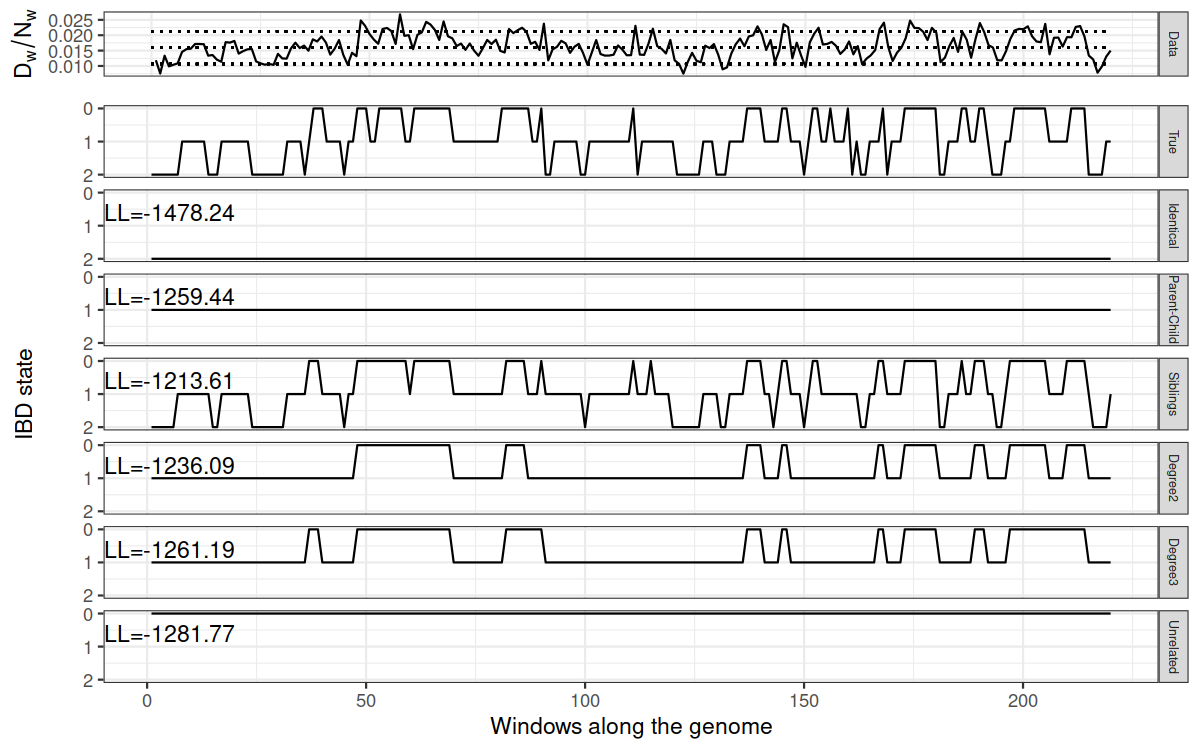
\includegraphics[width=16cm]{plots/plotimg/IBDplot.png}
    \centering
    \caption{Comparison of pairwise difference data and inferred IBD fragments. The top panel shows the proportion of differences in each window along the genome for a pair of simulated siblings. Dashed lines represent $p_0$, $p_1$ and $p_2$ estimates. The second panel shows the true IBD state for each window. The remaining panels show the IBD states predicted by particular relatedness models. The log likelihood value for each model is shown on upper left corner of the panel. Light and shaded background represent distinct chromosomes.}
    \label{fig1:ibd}
\end{figure}



\paragraph{Overview of simulations} 
We simulated an ancient population (sampled from 2500 generations ago) with msprime \cite{kelleher_efficient_2016}, and artificially mated some of the individuals to form a pedigree (figure \ref{figS10:pedigree}). We downsampled this data to low coverages (4$x$ - 0.03$x$), and applied KIN to find out a suitable cut-off for a reliable log likelihood ratio. We also introduced ascertainment bias and contamination from modern humans (see section \ref{method}) to test the performance of KIN, and compare it to that of READ. 
\paragraph{Critical Values}
 
 To investigate the limits of our method, we plotted the true-positive and false-positive rates when we use a particular difference in log-likelihood as a cutoff( fig. S \ref{figS10:cutoff}). The figure shows that for all relatedness cases except for $3^{rd}$-degree, the false positive rate is below $5\%$ even when simply selecting the model with the highest likelihood. We observe that for $3^{rd}$-degree relatives, using a cutoff of 1.0 brings down the false positive rate close to $5\%$ for all coverages except 0.05x. Thus, we  recommended to use a cutoff of 1 for all cases where ROH or contamination are not a concern.


\paragraph{Evaluating the ROH detection}
We next evaluate the performance of the ROH-HMM( Fig.\ref{fig2:ROH}). We observe that as coverage decreases, the raw heterozygosity estimates become more noisy. In the case without ROH (Fig \ref{fig2:ROH}A), we correctly infer that there is no ROH for all but two windows. We observe that the model predicts ROH probabilities well in all cases, even at a coverage of 0.1x (Table \ref{tab:Table 2}). 


\begin{figure}[h!]
    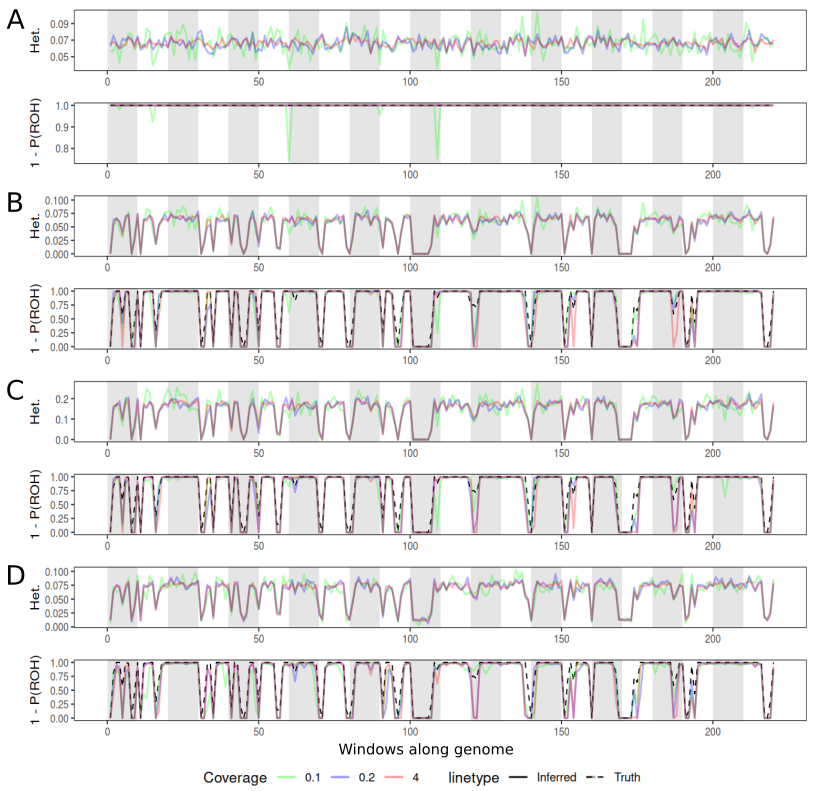
\includegraphics[width=16cm]{plots/inkscape_finalImg/ROHplot_final.png}
    \centering
    \caption{Estimation of ROH probabilities along the genome in simulations. Top panel shows proportion of differences in a simulated individual in windows along the genome, and the bottom panel shows probability of seeing no ROH. (A) Simulation with no ascertainment, contamination, or ROH. (B) Simulation with ROH. (C) Simulation with ROH and ascertainment. (D) Simulation with ROH and contamination.}
    \label{fig2:ROH}
\end{figure}

\paragraph{Comparing KIN-HMM with READ}
In Figure Fig. \ref{fig3:Comparison_READ_KIN}, we compare the classification accuracy of KIN (cutoff: 1 log-likelihood unit) to that of READ (cutoff: 1 standard deviation)  under four different simulation scenarios. We show that both methods have similar performance for low-coverage shotgun data (``control''-case), and for ascertained data. One exception is  $2^{nd}$-degree relatives, where KIN has higher power, especially at low coverages. We also find that READ is strongly impacted by contamination ($<3\%$), but that the correction implemented in KIN is sufficient to remove this bias. For simulations with ROH, we find the overall classification accuracy is only slightly reduced. Since ROH makes individuals more similar, we see a bias towards more false positives, for first and second-degree relationships, which is slightly higher for READ than for KIN.

\begin{figure}[h!]
    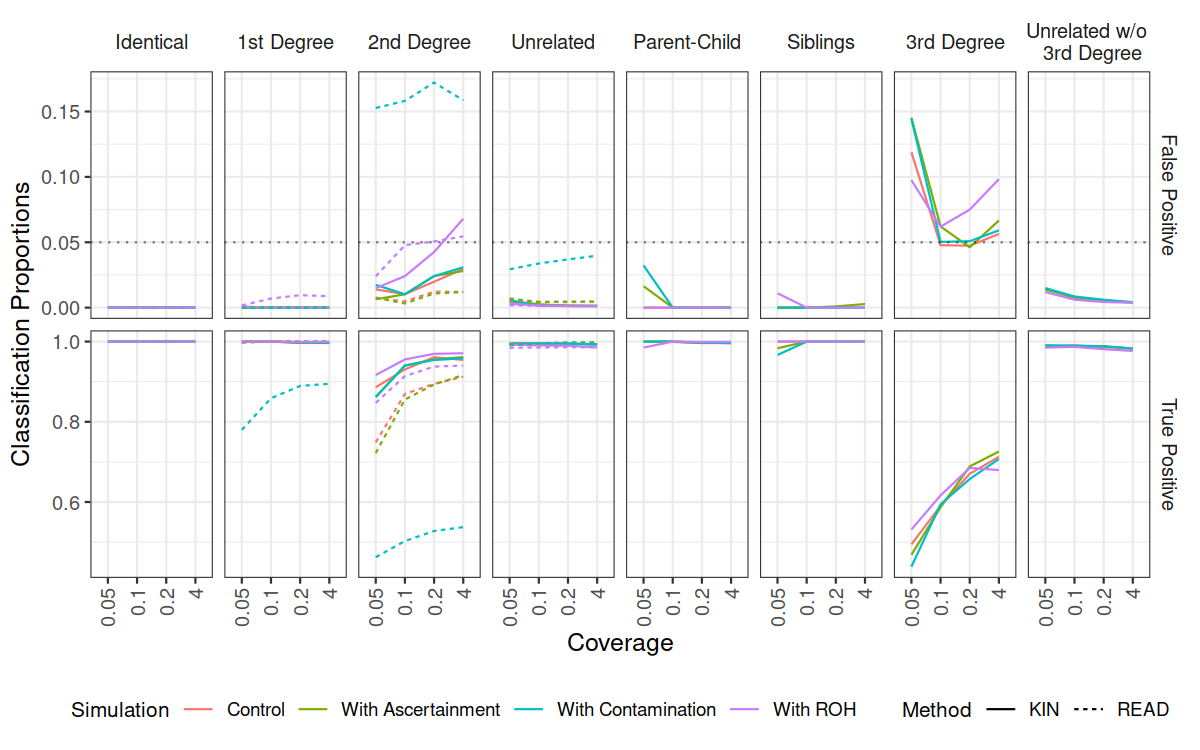
\includegraphics[width=16cm]{plots/plotimg/comparison_plot.png}
    \centering
    \caption{Comparison of KIN with READ using simulations with different coverages, and different cases of ascertainment, contamination and ROH. Unrelated label here refers to KIN performance results when all Unrelated, Fifth Degree, Fourth Degree, Third Degree pairs are labelled as Unrelated. 'Unrelated w/o $3^{rd}$ Degree' refers to the performance results when $3^{rd}$ Degree is classified separately from the unrelated individuals.}
    \label{fig3:Comparison_READ_KIN}
\end{figure}

\paragraph{Evaluating IBD prediction}
KIN co-estimates IBD states and relatedness, and hence it has a higher power to classify $2^{nd}$ degree relatives, and can distinguish between Siblings and Parent-Child. We investigate our limit to predict IBD states along the genome by calculating the number of genomic windows where we correctly  predict IBD state for a pair of individuals. We calculate mean and standard deviation for this accuracy over 60 simulations of a pedigree (see section \ref{simulat}). Fig. \ref{fig4:IBDstate_accuracy} shows that we can predict IBD states for Unrelated, $3^{rd}$ Degree, $2^{nd}$ Degree, and Sibling pairs very well at high coverages, and our accuracy decreases with downsampling. On the other hand, our accuracy measure for Identical individuals and Parent-Child remains very high, due to robust relatedness estimates for these cases even at 0.03x coverage depth.  


\begin{figure}[h!]
    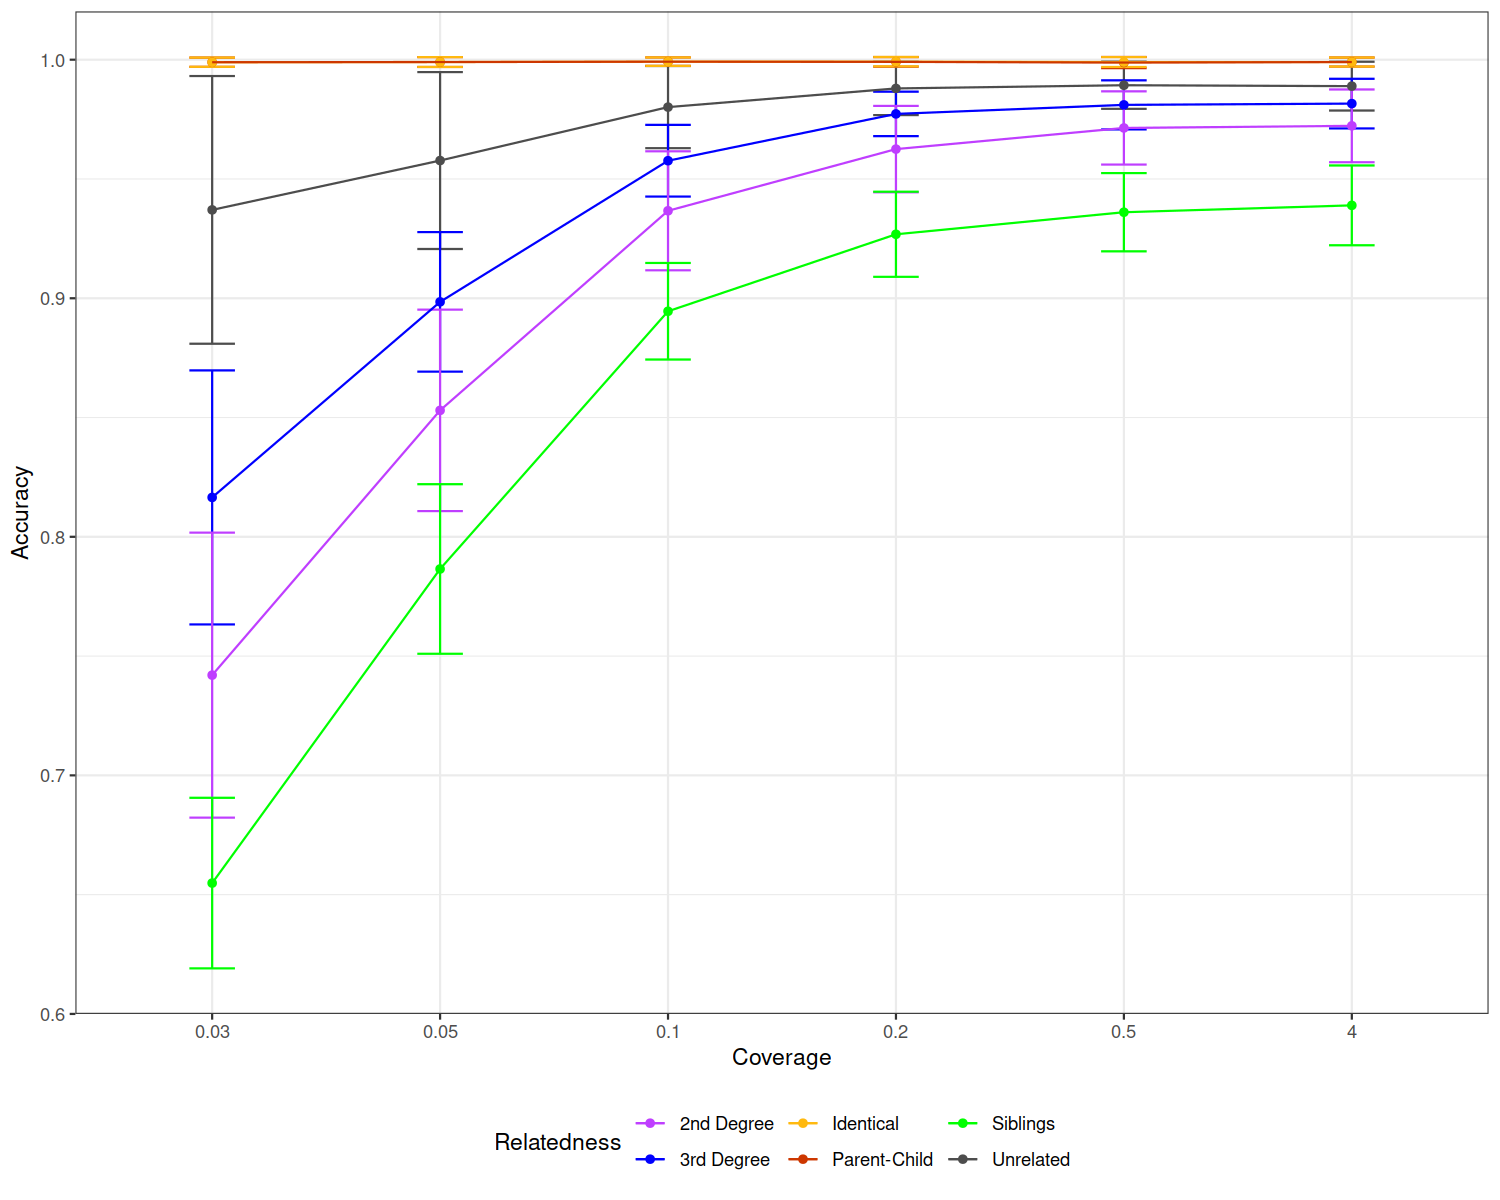
\includegraphics[width=16cm]{plots/plotimg/plot_IBDaccuracy.png}
    \centering
    \caption{Evaluation of IBD estimation at different coverages. y-axis shows accuracy calculated over 60 simulations with each relatedness case and six different coverages shown on x-axis. The error bars are drawn at 1 standard deviation from the mean. Here, accuracy corresponding to relatedness cases for Parent-Child and Identical individuals is always 1, and overlaps with each other.}
    \label{fig4:IBDstate_accuracy}
\end{figure}


\subsubsection{Application to Chagyrskaya Neanderthals}
To test KIN on real ancient data, we applied it to a Neandertal data set  from Chagyrskaya Cave in Siberia, Russia \cite{kolobova_archaeological_2020-1, mafessoni_high-coverage_2020}. This dataset contains genetic data from  14 skeletal remains that might  possibly belong to contemporary Neandertals who occupied the cave from 63 ± 4 to 48 ± 3 kya \cite{laurits_skov_genetic_nodate}. The data has low-to-intermediate depth of coverage ranging from 0.01x to 12.34x, with 8 samples at  $<1x$ coverage. Some of these specimens showed signs of long ROH, and contamination from modern humans as well as hyenas \cite{laurits_skov_genetic_nodate}. All these samples were captured with an array targeting for variable sites in high coverage Neandertal and Denisovan genomes, and common variations in Africans \cite{laurits_skov_genetic_nodate}. We further restricted this data to the variable sites in two high-coverage Neandertal genomes: Altai Neandertal (Denisova 5) \cite{prufer_complete_2014} and Vindija 33.19 \cite{prufer_high-coverage_2017} to make the data for our relatedness analysis same as that used by the authors. Our results for pairwise relatedness for these individuals is shown in Fig.\ref{fig5:Chagyrskaya_KIN}. We found three fossils from the same  individual (Chagyrskaya13-Chagyrskaya19-Chagyrskaya1141), a parent-child pair  (Chagyrskaya07 and Chagyrskaya17), and a pair of  $2^{nd}$-degree relatives (Chagyrskaya01/Chagyrskaya60). Further, we identify Chagyrskaya 07 and Chagyrskaya 60 as 3rd-degree relatives. 

Our estimates are consistent with those obtained using READ, except that READ is unable to detect 3rd-degree relationships, and cannot distinguish between siblings and parent-child. We also find that both  KIN and READ classify Chagyrskaya06 and Chagyrskaya14 as parent-child with low confidence, but from the morphology they likely stem from the same individual. We believe that the low confidence miss-classification arises  due to non-human contamination present in these libraries ($1\%$ and $2.9\%$ respectively \cite{laurits_skov_genetic_nodate}), biasing the estimated differences between the individuals to higher values.

We compared our IBD estimates to lcMLkin for all pairs for whom READ results (with s.d. $>$1) and KIN results ($\Delta LL>$1) match (fig. S\ref{figS6:Chagyrskaya_ibd}). We find that lcMLkin does create four different clusters for different relatedness cases. However, the location of these clusters strongly deviate from the expected values, likely due to the low coverage and ROH. Remains from the same individual, for example, are expected to be at $k_0 = 0$ and $r = 1$, but are at $k_0 \approx 0.33$, $r \approx 0.6$.


\begin{figure}[h!]
    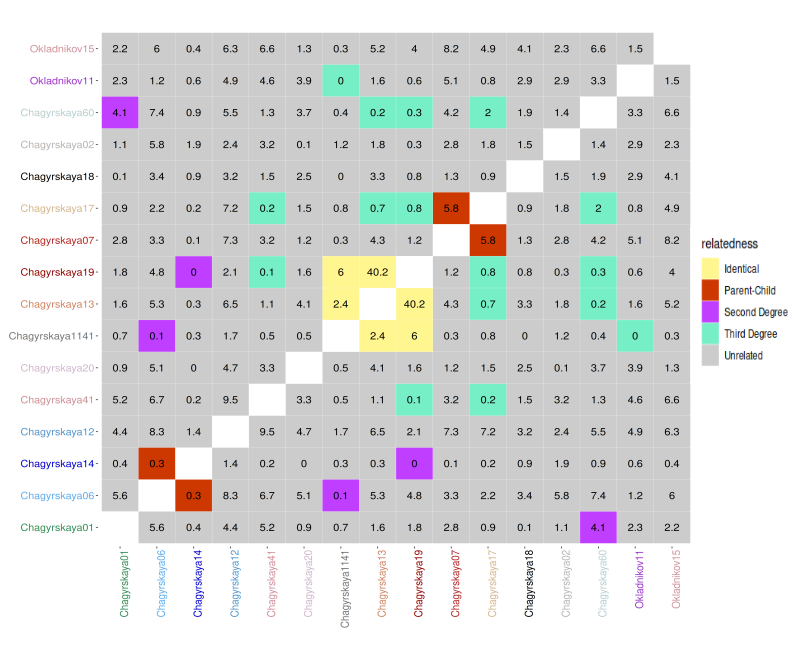
\includegraphics[width=18cm]{plots/inkscape_finalImg/kinplot.png}
    \centering
    \caption{Application of KIN on Neandertal specimens from Chagyrskaya. The color of a square represents the relatedness, while the number within denotes log likelihood ratio ($\Delta LL$) between the two maximum likelihood models.}
    \label{fig5:Chagyrskaya_KIN}
\end{figure}

We further applied KIN to a genome-wide dataset of 118 ancient individuals from the Lech Valley \cite{mittnik_kinship-based_2019}. We compared our relatedness estimates to those obtained by the authors using READ and lcMLkin, and found that in most cases the three methods agree. Out of 6903 pairwise comparisons, 346 pairs show different relatedness for KIN and READ (table S2). However, most of these are at very low confidence, and there are only 31 pairs where KIN has $\Delta LL>1$. When we investigated these comparisons in more detail we found that in many cases, the proportion of differences along the genome align with the prediction by KIN (fig. S\ref{figS8:eg1}). Only 20 pairs in this subset of 346 pairs had sufficient data for analysis using lcMLkin (more than 10,000 overlapping SNPs). Among these 20 pairs, we found that lcMLkin matches KIN's estimate in all cases except for pair POST131-POST28 (READ predicts unrelated individuals, lcMLkin predicts 3rd-5th degree, KIN predicts second degree) and pair AITI72-AITI77A (READ and lcMLkin predict unrelated, while KIN estimates 3rd degree with LL=1.7).  
We further found 43 pairs for which READ estimates First-Degree, and compared the estimates of lcMLkin and KIN for these cases (Table S3). There were a total of 20 pairs where lcMLkin had sufficient data, and 26 pairs where $\Delta LL>1$ for KIN. Among the 19 overlapping pairs, we found four pairs where KIN and lcMLkin differ, and again the heterozygosities along the genome match the inference of KIN (fig. S\ref{figS9:eg2}).  


\section{Discussion}\label{discussion}
Here, we present a new method called KIN to estimate genetic kinship and the location of IBD tracts from low-coverage data, in presence of long ROH, contamination, as well as ascertainment bias. Our method utilizes a set of HMMs to estimate IBD tracts and uses them to classify each pair of individuals into a possible relatedness case, along with a measure of classification confidence. We evaluated the method performance of KIN, and compared it to that of READ using simulated pedigrees. Finally, we show applications of KIN on two ancient datasets.


In our simulations, we find that adding long ROH ($~17\%$) to simulations slightly improves the performance of both KIN and READ, particularly at lower coverages. This is likely because ROH actually reduces the variance in differences, and so it becomes easier to estimate the location of IBD tracts. For READ, the presence of ROH causes a bias towards inferring closer relatedness cases, but the model we use in KIN reduces this bias (see Fig. \ref{fig3:Comparison_READ_KIN}). 

Contamination can affect the accuracy of relatedness inference for two reasons. For one, if a substantial fraction of samples is contaminated, then the estimation of $p_0$ becomes inaccurate, because the majority of pairwise differences will include at least one contaminated sample. The second issue is that contaminated samples will look less similar to other individuals, and thus cause a bias towards inferring them to be less related to other individuals. The amount of contamination does not need to be large for this to be important, in our simulations we find that even at contamination levels $\leq 3\%$, the performance of READ is substantially reduced. Assuming the contamination rates are correctly inferred, the correction we implemented leads to improved performance compared to naive methods such as READ, although they too could be ameliorated in a similar way \cite{laurits_skov_genetic_nodate}. SNP ascertainment can cause a slight decrease in power for both  methods, since it reduces the amount of data available. However, the decrease in power is lower for KIN compared to READ.

The Lech Valley data  has low contamination, and no ROH. For pairwise comparisons with large numbers of overlapping sites ($>10000$), KIN, READ and lcMLkin all mostly agree. However, KIN is able to differentiate between parent-child and siblings, and identify second and third degree relationships from just a few thousand sites overlapping between samples. We show that when applied to Neandertal specimens from Chagyrskaya Cave, KIN identifies a pair of $1^{st}$-Degree relatives as parent-child, which is in agreement with the finding that the mtDNA haplotypes differ between the samples \cite{laurits_skov_genetic_nodate}. In addition, KIN identifies a pair of $3^{rd}$ degree relatives. In this case of a population with large amounts of ROH, we find that the inference by lcMLkin are heavily biased, but KIN's model takes ROH into account and both the coefficient of relatedness and $k_0$ are very close to what would be expected from the inference by both READ and KIN. 

One limitation of our approach is that it assumes a single population. In case of a highly structured population, KIN may show inaccurate inferences, similar to READ and lcMLkin. Also, our method makes the assumptions, that the median pairwise genetic difference reflects the population diversity, which fails if almost all individuals in the data set are related. The current implementation of KIN is restricted to six relatedness cases we expect to be most common, but it might be feasible to extend it to other cases, such as double first cousins, using a corresponding IBD state transition matrix.

While we have focused on the application of KIN on ancient human samples, the model is not tied to this system. Assuming we know the recombination rate, and hence can estimate the transition matrix (see section \ref{method}), KIN can be widely applied to any diploid species. In addition, the output of KIN is a table which shows for each pair, the most likely model, and the second best guess, along with a confidence level represented by the log likelihood ratio. This makes KIN easy to automatize for large datasets. To make application of KIN user-friendly, we provide a python package to create input files for KIN from processed bamfiles, while optionally estimating ROH, and correcting for contamination estimates. 


\section{Materials and methods}\label{method}

\subsection{Simulations}\label{simulat}
We use simulations both for estimating the transition matrices and for testing and validating our algorithm. All simulations are performed in a scenario mimicking the analysis of a Neandertal population contaminated by modern humans. We simulate unrelated individuals using $\texttt{msprime}$ \cite{kelleher_efficient_2016}, followed by an additional step where we simulate related individuals using a predetermined pedigree (Figure S\ref{figS10:pedigree}).

\paragraph{Simulating pedigrees}

For our simulations of background diversity, we form a population (Pop1) with constant effective size of 10,000 and sample eight diploid individuals (each made up of two haploid individuals) from 2500 generations ago (fig. S \ref{figS10:pedigree}). For each individual, we simulate 22 chromosomes with length $L=100$ Mb and a recombination rate of $r=10^{-8}$ per base pair per generation. We introduce mutations using an infinite sites model with rate  $\mu= 10^{-8}$ per base pair per generation. 

For the pedigree simulations, we first simulate a recombined set of chromosomes for either parent, and combine them to create the progeny. We simulate recombination by first drawing the number of breakpoints as a  Poisson random variable with parameter $rL$, and use a uniform distribution on $[1, L]$ to sample the positions of recombination points. The pedigree simulations result in nine addition individuals, resulting in a total sample of 17 individuals.

\paragraph{Transition matrices}
KIN requires a transition matrix for each relatedness case. which we estimate  by counting the transition between IBD states for all pairs of individuals at that relatedness level in a training set of 1000 simulations from our pedigree (Fig. S \ref{figS10:pedigree}). For two cases, siblings and grandparent-grandchild, it is possible to write down the theoretical expectation of the transition matrix: 

For grandparent-grandchild, rate matrix is
 $$Q = \left[\begin{array}
{rrr}
-r & r \\
r & -r 
\end{array}\right]$$   

Here the state space includes only $Z_w=0$ and $Z_w=1$. 
Similarly, for a pair of siblings, we calculate $$Q =  
\left[\begin{array}
{rrr}
-4r & 4r & 0\\
2r & -4r & 2r\\
0 & 4r & -4r
\end{array}\right]$$   

The state space includes all IBD states in this case. For these two cases, we get the transition matrix in each case as $e^{Qb}$, where b is the window size.


\paragraph{Simulations for method evaluation}
Apart from the related and unrelated individuals in Pop1, we simulated more haploid individuals in three other populations to create scenarios with ascertainment bias and contamination (fig. \ref{figS10:pedigree}). We simulated two individuals to form an individual each from two other populations (Pop2, Pop3) with split time of 3500 and 4500 generations with Pop1, and sampling time of 4000 generations and 2000 generations ago respectively.  We identified the sites that were polymorphic among these two individuals, and used these sites to ascertain the genomes of individuals from Pop1. This scenario roughly models the ascertainment of the Chagyrskaya data. We tested the performance of our method in presence of long ROH ($\sim17\%$), by simulating regions of homozygosity with a Markov chain using the transition matrix

$$\mathbf{A} = \left[\begin{array}
{rr}
1-10/L & 10/L \\
2/L & 1-2/L  \\
\end{array}\right]
$$

From the steps described above, we got genotypes of individuals in Pop1 in presence/absence of ROH and ascertainment. We further simulated five diploid individuals from Pop4 with split time of 20,000 generations with Pop1, sampled from the present time, as a source of contamination.  For cases including contamination, we contaminated eight individuals with varying amounts between 0.5\% to 3\% contamination, with the remaining  nine individuals did not have any contamination. We generated reads (derived/ancestral) for different genomic coverages ranging from 4x to 0.03x, assuming a Poisson distribution.

For testing, we replicate each simulation 60 times, and create data from the same base simulations at varying levels of coverages and different scenarios: We have a control scenario (without ascertainment bias, ROH or contamination), and individual scenarios where we add ROH, SNP ascertainment and contamination, respectively. For the evaluation of the ROH-HMM, we also combine ROH with ascertainment or contamination.

\renewcommand\thefigure{\arabic{figure}}    
\section{Supplementary Information}
\setcounter{figure}{0}   


\begin{table}
\caption{\label{tab:Table 2}Model performance for ROH prediction. Here we test ROH-HMM in four different cases of simulations: Control (without ROH, ascertainment bias or contamination, R (with ROH), RA (with ROH and ascertainment bias), RC (with ROH and contamination)}
\begin{tabular}{|c|c|c|c|c|c|c|c|c|}
    \hline
    Coverage & Control(bias) & Control(var) & R(bias) & R(var) & RA(bias) & RA(var) & RC(bias) & RC(var)\\
    \hline
    4x & -0.007 & 0.006 & -0.081 & 0.036 & -0.083 & 0.036 & -0.091 & 0.039\\
    \hline
    0.2x & -0.003 & 0.003 & -0.068 & 0.03 & -0.068 & 0.026 & -0.076 & 0.029\\
    \hline
    0.1x & -0.003 & 0.002 & -0.049 & 0.021 & -0.05 & 0.021 & -0.057 & 0.022\\
    \hline
\end{tabular}
\label{table1}
\end{table}

\renewcommand{\figurename}{Fig. S}
\begin{figure}[h!]
    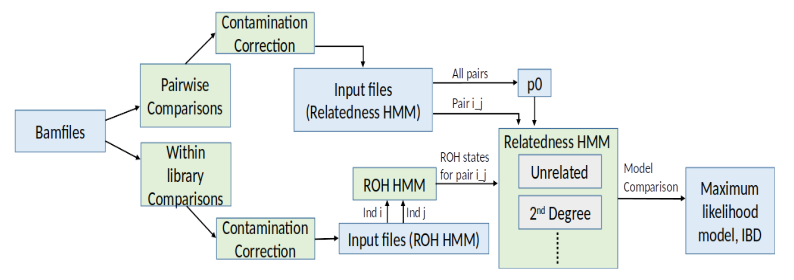
\includegraphics[width=18cm]{plots/inkscape_finalImg/schematic_sup.png}
    \centering
    \caption{Overall schematic of the method showing the entire pipeline from processed bam files to final relatedness and IBD estimates. Blue boxes show the data files, while green boxes represent scripts.}
    \label{figS0:schematic}
\end{figure}




\begin{figure}[h!]
    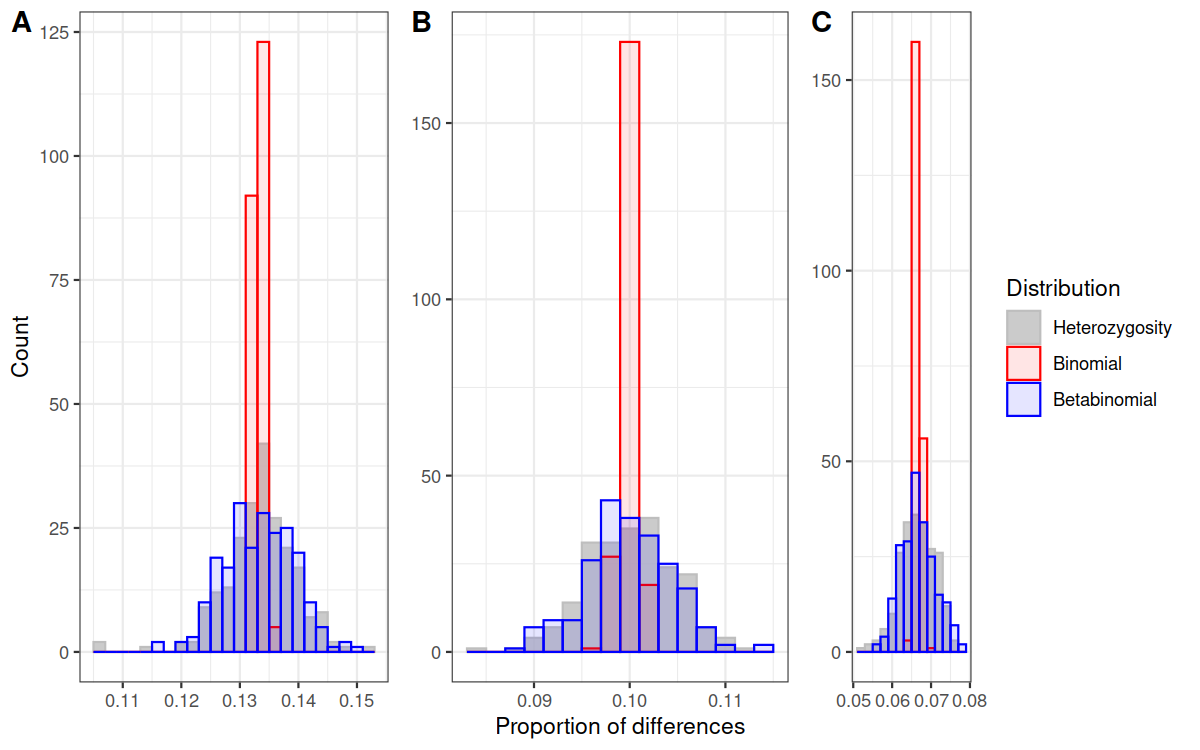
\includegraphics[width=18cm]{supplementary_info/plots/binom.png}
    \centering
    \caption{Comparison of fit with Beta-binomial and Binomial distributions. Data is represented by the histogram of proportion of differences from all windows of a (A) unrelated, (B) Parent-Child, (C) Identical pair of individuals. Binomial parameter p is calculated from the data, while Beta-binomial parameters are estimated with the relatedness HMM.}
    \label{figS1:binom}
    
\end{figure}


\begin{figure}[h!]
    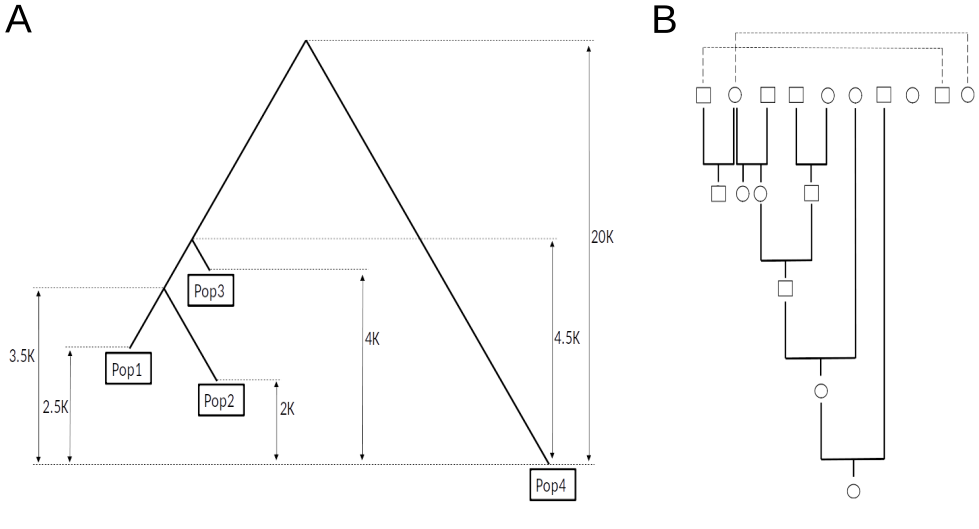
\includegraphics[width=18cm]{plots/inkscape_finalImg/pedigree_both.png}
    \centering
    \caption{Overview of simulated dataset. (A) We simulated four different populations with split times and sampling times (in generations) mimicking the populations of Chagyrskaya Neandertals, Vindija Neandertals, Altai Neandertals and present day Africans \cite{mafessoni_high-coverage_2020}. We artificially mated individuals in Pop1 to create related individuals. We used Pop2 and Pop3 to introduced ascertainment bias in the data, while we simulated contamination from modern humans using Pop4. (B) In Pop1, we sampled 8 diploid unrelated individuals, and artificially mated some of them to make a pedigree with upto $5^th$ Degree relatives. Circles represent females, and squares represent males. Dotted lines connect identical pair of individuals.}
    \label{figS10:pedigree}
    
\end{figure}


\begin{figure}[h!]
    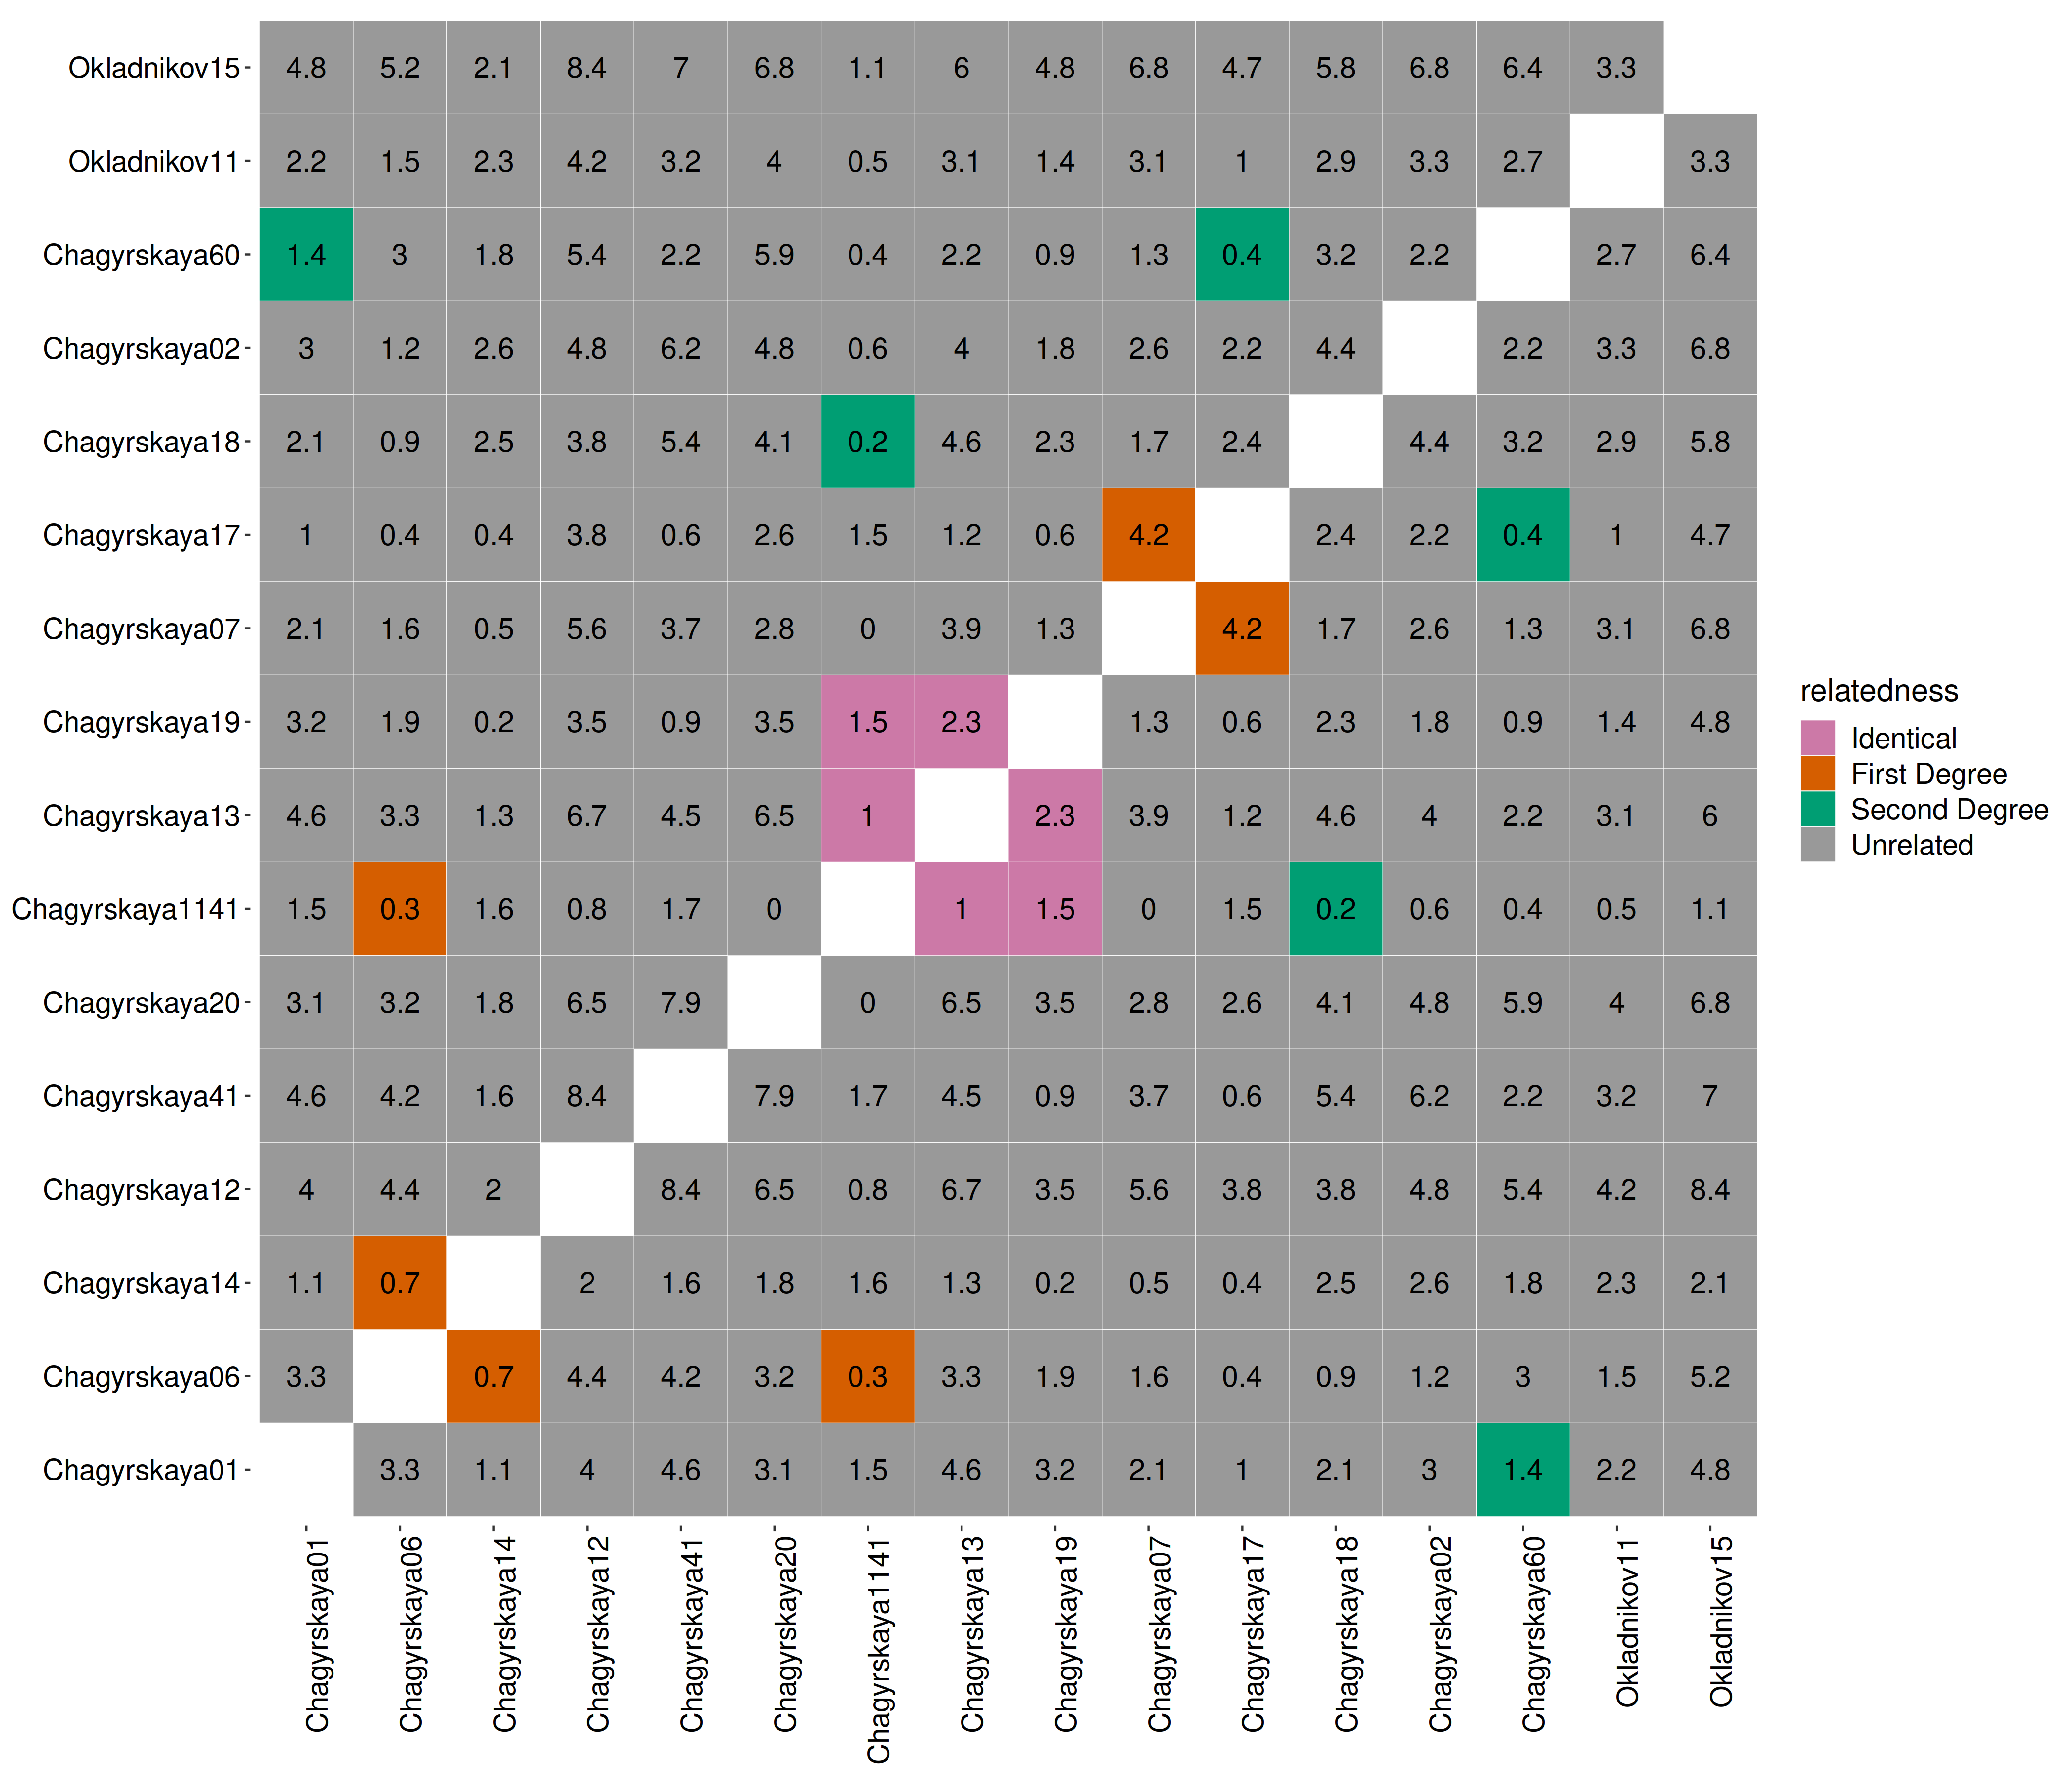
\includegraphics[width=18cm]{supplementary_info/plots/fil0_read_plot.png}
    \centering
    \caption{Application of READ on Neandertal specimens from Chagyrskaya Cave. Color of a square represents the relatedness, while the number denotes standard deviations away from the upper threshold (we show lower threshold for unrelated pairs since upper threshold is not available).}
    \label{figS2:Chagyrskaya_READ}
\end{figure}


\begin{figure}[h!]
    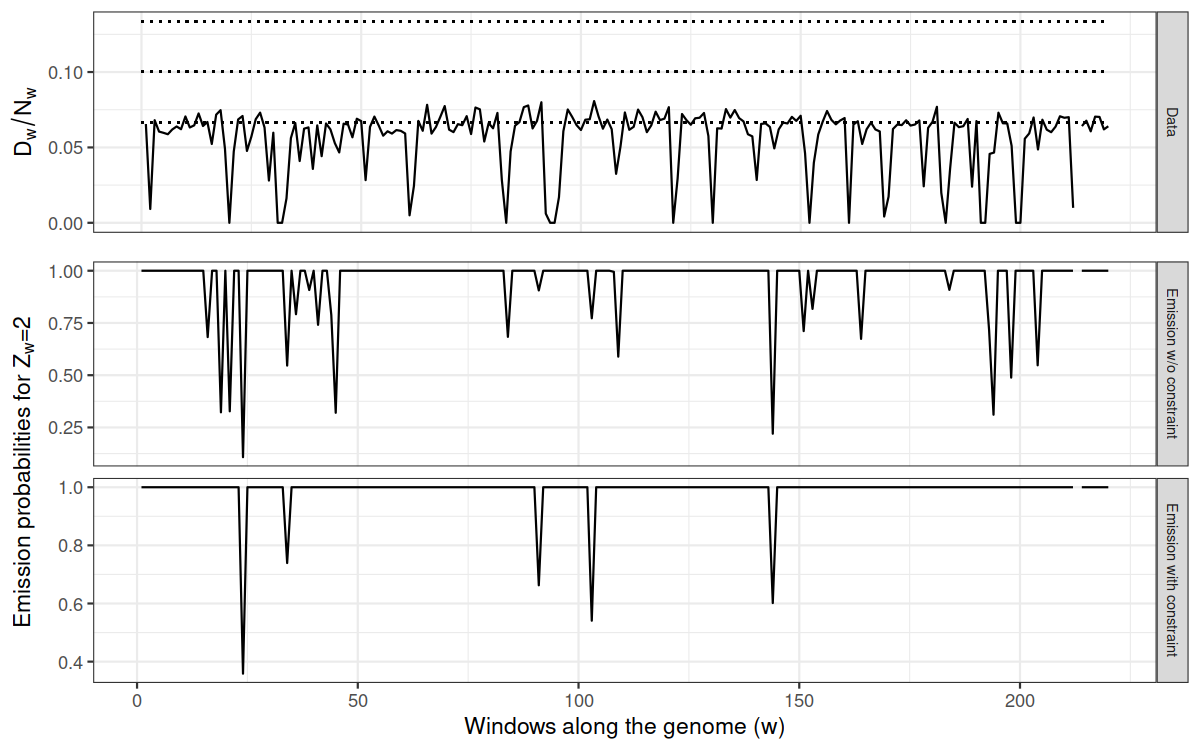
\includegraphics[width=18cm]{supplementary_info/plots/contam0_inbred1_run57_coverage0.2_asc0_inputMode_hapProbs_fil0_pair0_15_relid_emissions_bnds.png}
    \centering
    \caption{Application of identical relatedness HMM on a pair of identical individuals with low coverage (0.2x), and ROH tracts. Top panel shows pairwise proportion of differences is close to expectation, but dips in some windows due to presence of ROH tracts. Bottom two panels show $P(Data|Z_w=2)$ without constraints and with constraints respectively.}
    \label{figS3:bnds}
\end{figure}



\begin{figure}[h!]
    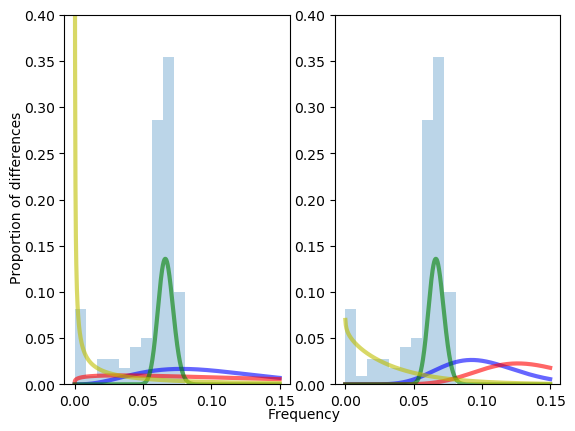
\includegraphics[width=18cm]{supplementary_info/plots/contam0_inbred1_run57_coverage0.2_asc0_inputMode_hapProbs_fil0_pair0_15_relid_betaplot.png}
    \centering
    \caption{Comparison of beta distributions estimated with the KIN-HMM (left) without and (right) with variance constrained optimization of $\delta$ parameters.The histogram in each plot shows pairwise differences in genomic windows. Colored lines shows the Beta probability distribution for each IBD state $Z_w$.}
    \label{figS4:bndsbeta}
\end{figure}


\begin{figure}[h!]
    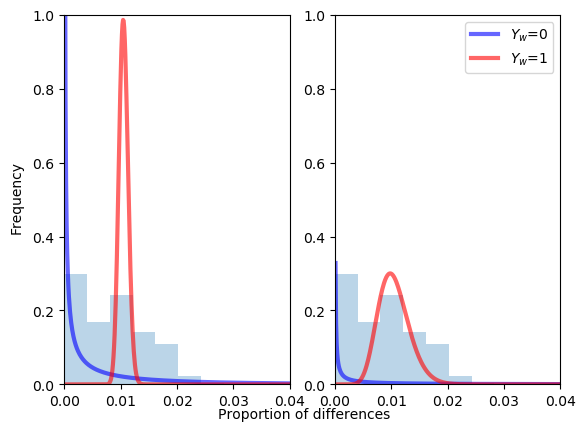
\includegraphics[width=18cm]{supplementary_info/plots/contam0_inbred1_run57_coverage0.2_asc0_inputMode_hapProbs_fil0_ind0_forced_roh.png}
     \centering
    \caption{Comparison of Beta distributions estimated with ROH-HMM (left) without and (right) with constrained emissions. The histogram in each plot shows pairwise differences in genomic windows. Colored lines shows the Beta probability distribution for each homozygosity state $Y_w$.}
    \label{figS5:ROHforced}
\end{figure}

\begin{figure}[h!]
    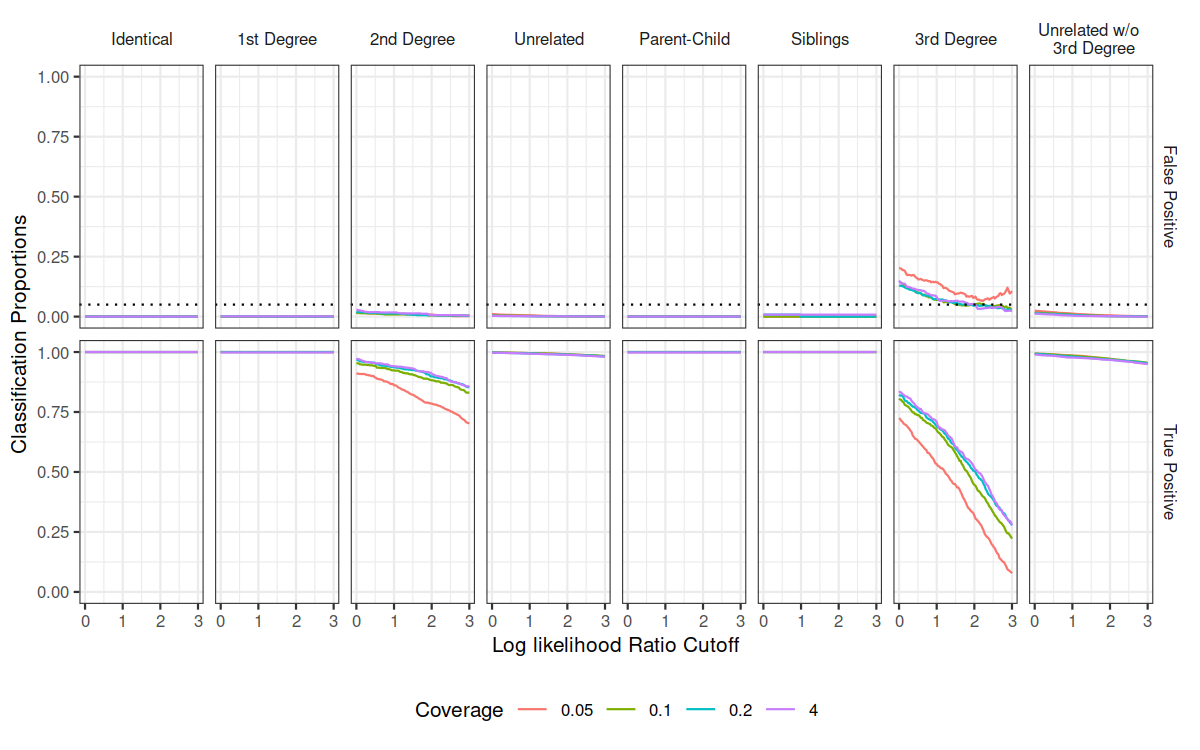
\includegraphics[width=16cm]{plots/plotimg/contam0_inbred0_model_performance_allroc_asc0_plot.png}
    \centering
    \caption{False positive and true positive rates as a function of cutoff on log likelihood ratio. In top panel, dotted line represents $5\%$. Unrelated label here refers to KIN performance results when all Unrelated, Fifth Degree, Fourth Degree, Third Degree pairs are labelled as Unrelated. 'Unrelated w/o $3^{rd}$ Degree' refers to the performance results when $3^{rd}$ Degree is classified separately from the unrelated individuals.}
    \label{figS10:cutoff}
\end{figure}



\begin{figure}[h!]
    \centering
    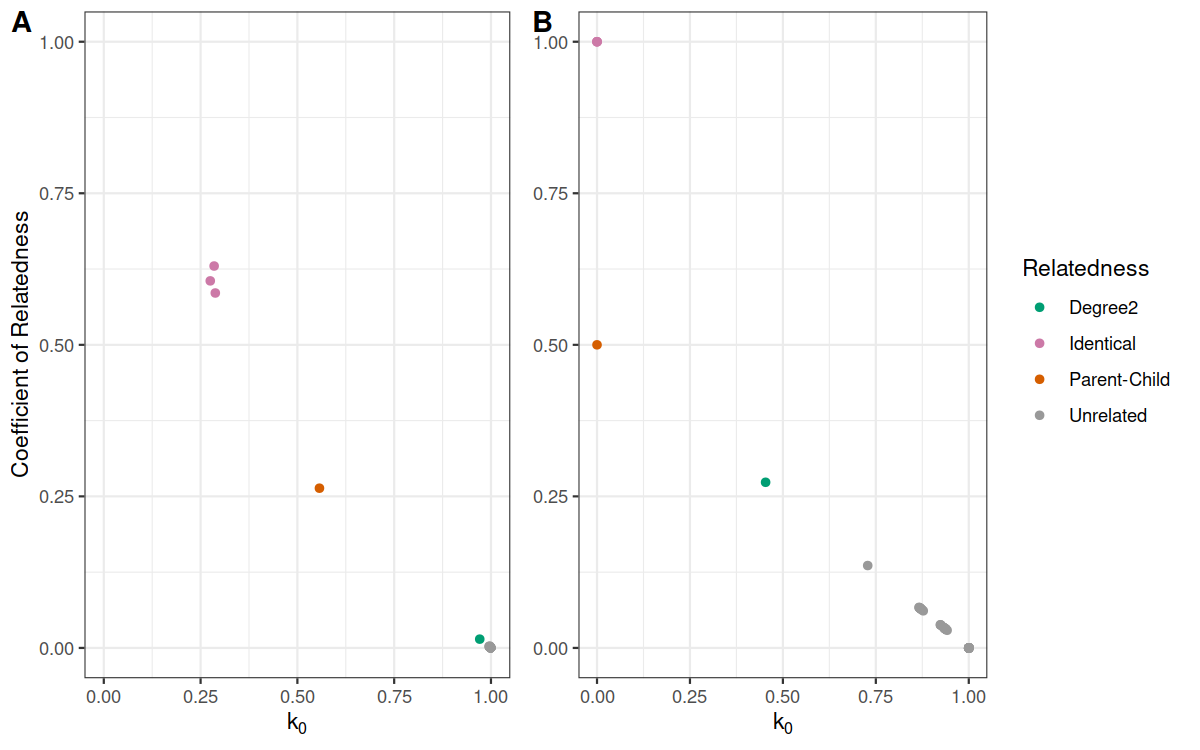
\includegraphics[width=18cm]{supplementary_info/plots/lcPlot.png}
    \caption{Comparison of IBD states estimated for Chagyrskaya specimens using (A) lcMLkin and (B) KIN. Each plot shows relatedness coefficient (calculated as $k_2+k_1/2$) on y-axis plotted against $k_0$ (proportion of genome with no chromosomes shared).
    The relatedness shown with different colors is estimated with both READ and KIN.}
    \label{figS6:Chagyrskaya_ibd}
\end{figure}


\begin{figure}[h!]
    \centering
    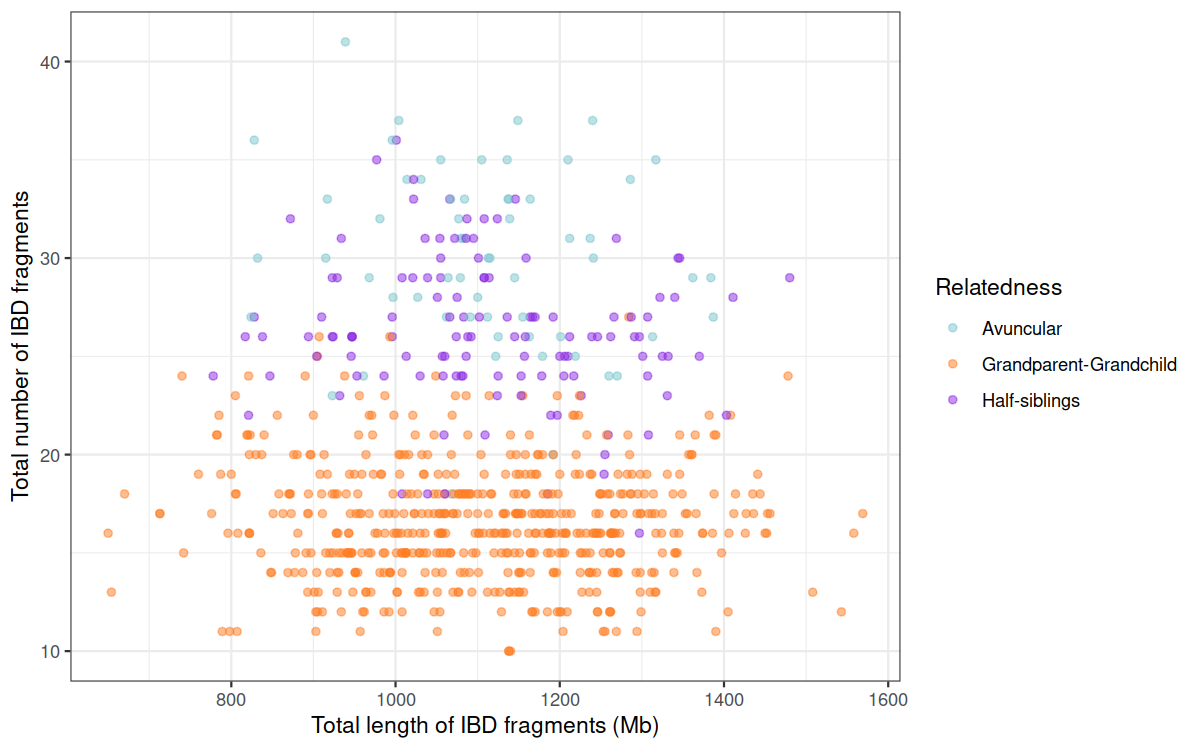
\includegraphics[width=18cm]{supplementary_info/plots/degree2_10Mwin.png}
    \caption{Plotting total number of IBD fragments with the number of IBD fragments can tease apart avuncular relationship from grandparent-grandchild, since they form different clusters. Half-siblings, however, overlap considerably with both these relations.}
    \label{figS7:second_degree}
\end{figure}


\begin{figure}[!ht]
    \centering
    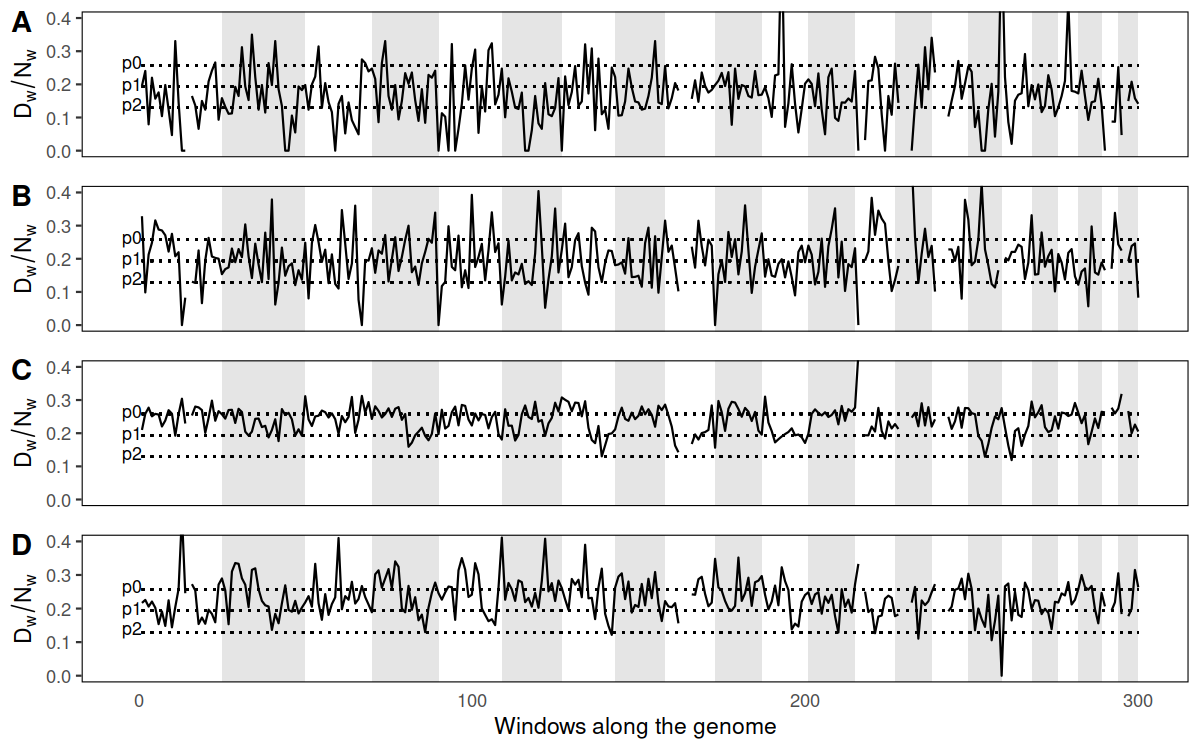
\includegraphics[width=18cm]{supplementary_info/plots/egplot1.png}
    \caption{Plots showing proportion of differences in windows along the genome for some of the pairs of relatives for which KIN differs from READ. (A) AITI62B-OTTM156 (READ estimates Identical individuals, lcMLkin does not have sufficient data, and KIN predicts parent-child. (B) UNTA5867-UNTA5868Sk1 (READ estimates Second Degree, lcMLkin does not have sufficient data, and KIN predicts parent-child). (C) AITI40-AITI72 (READ estimates Unrelated individuals, lcMLkin shows 3rd-5th degree, and KIN predicts 3rd degree.)
    (D) AITI2-AITI55 (READ estimates Unrelated individuals, lcMLkin and KIN predicts predict second degree.)}
    \label{figS8:eg1}
\end{figure}

\begin{figure}[h]
    \centering
    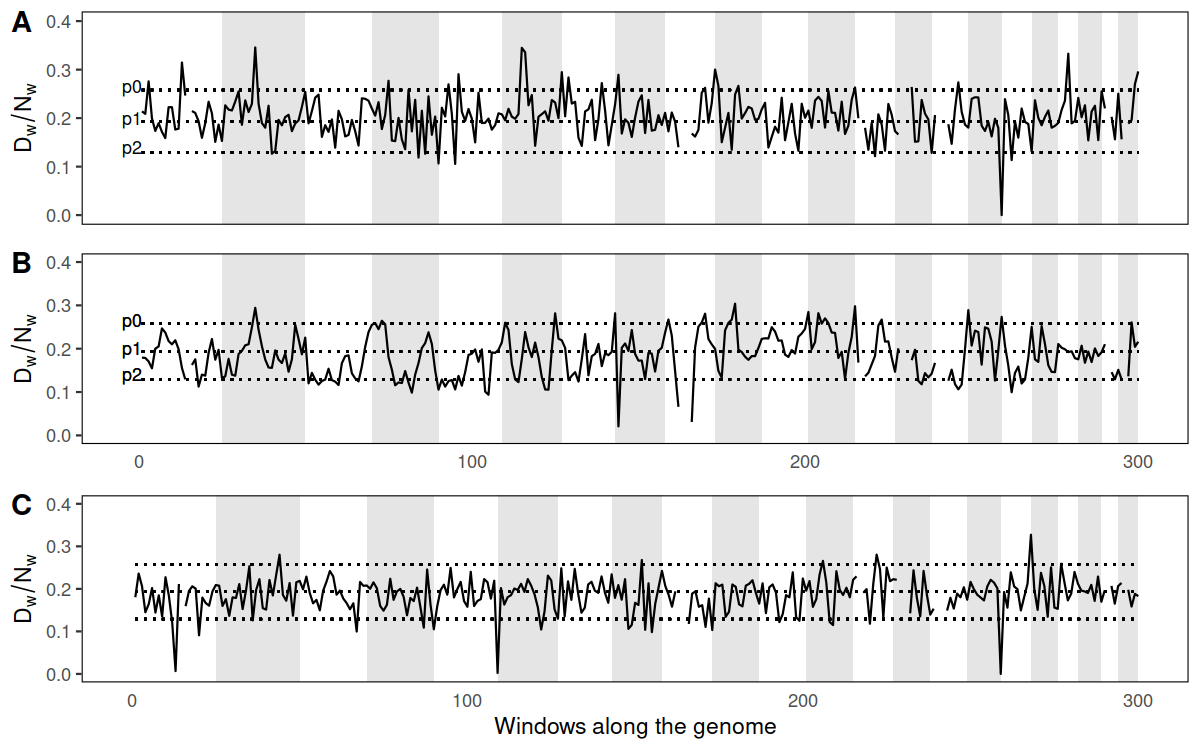
\includegraphics[width=18cm]{supplementary_info/plots/egplot2.png}
    \caption{Plots showing proportion of differences in windows along the genome for some of the pairs of relatives for which KIN differs from lcMLkin. (A) AITI43-AITI55 (READ estimates First degree, lcMLkin predicts siblings, while KIN predicts parent-child. (B) AITI70-AITI72 (READ estimates First degree, lcMLkin predicts parent-child, while KIN predicts siblings.}
    \label{figS9:eg2}
\end{figure}

\bibliographystyle{plain}
\bibliography{references.bib}

\end{document}

